The work in this section was published in \textcite{Walter_flexcable}. 

\subsection{Introduction to Cryogenic Microwave Wiring}
Microwave interconnects that span from room temperature to sub-Kelvin temperatures are required for large arrays of superconducting devices. Low transmission loss before amplification and digitization is required for highly sensitive detectors. As device arrays increase in size, thermal conduction along the electronic leads dominates the heat load on the cold stage of the cryogenic refrigerator. It is common to use superconducting coaxial cables below 4~K but these quickly become unwieldy in large numbers within a cramped cryostat and their large cross sections result in unacceptable heat loads for adiabatic demagnetization refrigerators (ADRs). Planar transmission line circuits on a flexible substrate naturally organize multiple lines and their shared ground plane reduces the thermal cross section. There are several examples of cryogenic ribbon cables for DC voltages at millikelvin temperatures \parencite{Woodcraft, Yung} and for frequencies spanning 1--20~GHz down to 4~K \parencite{Harris, McGarey}. A large effort has been made in depositing polyimide and metal on a substrate wafer before performing a liftoff to create flexible circuits with Al, Nb, NbTi, and YBCO superconductors \parencite{Paik, Allen, vanWeers, Pappas, Tuckerman}. Scalable, high density, low loss, broadband microwave interconnects for millikelvin temperatures are motivated by large arrays of sensitive cryogenic devices currently under development such as quantum computing qubits \parencite{Martinis}, X-Ray microcalorimeters \parencite{Ulbricht}, sub-millimeter bolometers \parencite{SCUBA2}, nanowire single-photon detectors \parencite{Verma, Bellei}, and broadband Microwave Kinetic Inductance Detectors (MKIDs) \parencite{NIKA2, MUSIC, ARCONS, Meeker2018}.

We developed superconducting NbTi microstrip flex cables specifically as broadband signal carriers for multiplexed 10,000+ sensor MKID arrays for astronomy operating at 100~mK \parencite{Meeker2018, PICTURE-C}. These cables are unique in that they target low loss up to 10 GHz, working temperatures between 0.1--4~K,  reduced complexity with push-on connectors, and lengths up to 40~cm limited by the standard commercial panel size. Our process laminates a 53~wt\%~Nb~-~47~wt\%~Ti (Nb-47Ti) alloy foil to an adhesive/polyimide panel stackup, etches a microstrip pattern into the top metal layer, and laser cuts the flex cables from the panel. This design and fabrication is detailed in Section \ref{sec:flexcable} along with the G3PO coaxial interface. We present transmission loss and crosstalk measurements at 30 mK in Section \ref{sec:measurements} and compare with an analytical model and simulations made with Sonnet Suites planar EM software. While we have not directly measured the thermal conductivity, in Section \ref{sec:thermal} we use published data to estimate the thermal load on a 0.1~K stage from 0.8~K for microstrip flex cables in an ADR and compare to commercially available superconducting coaxial cables. 

\subsection{Superconducting Flex Cable Design}
\label{sec:flexcable}
The flex cables were fabricated by Tech-Etch\footnote{Tech-Etch, Inc., 45 Aldrin Road, Plymouth, MA 02360 USA} using a proprietary thermal pressure lamination and wet etch process. They consist of Nb-47Ti foil sandwiching a dielectric stack up of Nikaflex CISV2525 and Hanwha HGB E250LP bisphenol epoxy. Nikaflex is a flexible DuPont/Nikkan coverlay film composed of 0.025~mm HFB-E250YG adhesive and 0.025~mm Kapton 100V. Nb-47Ti is superconducting below 10~K, is non-magnetic, and has relatively low thermal conductivity below 4~K compared to metals like Al, Nb, CuNi and SS alloys \parencite{DaalInPrep}. The first iteration uses 0.048~mm Nb-47Ti purchased and rolled by ATI\footnote{ATI Specialty Alloys \& Components, 1600 Old Salem Rd., Albany, OR 97321 USA} and 0.051~mm of the Hanwha HGB epoxy for a total stackup of 0.198~mm and is pictured in \figurename~\ref{fig:FlexCable}. In our second manufacturing trial Rikazai\footnote{Rikazai Co., LTD., 1810 Shimonumabe Nakahara-ku, Kawasaki City, Kanagawa Pref., Japan} rerolled the same Nb-47Ti to 0.010~mm thickness and we use only 0.025~mm thick Hanwha HGB epoxy for a total stackup of 0.096~mm. After lamination, the top metal layer is etched into parallel traces with a width of 0.2~mm each for a 50~Ohm impedance. Several designs were fabricated having up to 40~cm in length and up to 10 traces per cable. The flex cable tested for this paper is from our first iteration of cables having a thickness of 0.198~mm, 22~cm length, and 5 traces. We use a 3.556~mm trace pitch in order to match the standard package density of Corning Gilbert's G3PO connector (compatible with SMP-S).

Hand flectional stress tests indicate the cables will flex elastically for bends as small as 6.4~mm in radius and are robust to multiple cryogenic cooling cycles. Sharper bends, when repeated, can cause fractures in the Nb-47Ti traces. Thinner materials allow a smaller bending radius.

\begin{figure}[!t]
  \centering
	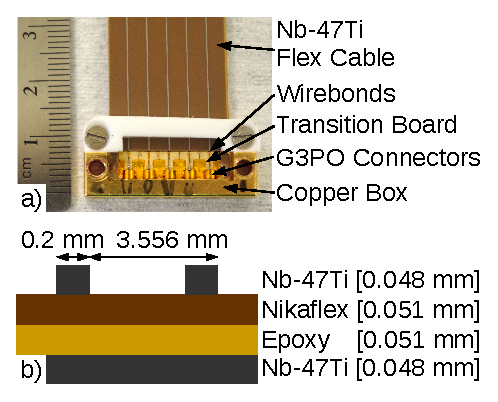
\includegraphics[width=8.5cm]{flex_stackup_MIR.eps}
  \caption[Flex cable design]{a) Image of assembled Nb-47Ti flex cable. b) Flex cable fabrication stackup with various thicknesses and dimensions indicated. Not to scale in horizontal direction.}
  \label{fig:FlexCable}
\end{figure}

Flex cable traces are connected to traces on a copper transition board with two 0.025~mm Al wire bonds. The transition board is a 0.254~mm thick RT/Duroid 6010LM PCB with 50~Ohm traces that start as microstrips and transition to a grounded coplanar waveguide (GCPW) geometry for increased signal isolation. G3PO surface mount connectors are soldered onto the GCPW side of the transition board and the whole end assembly is supported by a copper box. The flex cable is glued to the copper box with EPO-TEK EE129-A silver epoxy which is still conductive at cryogenic temperatures. The transition board and copper box with G3PO connectors allows for easy push-on coax interconnections between electronics and supports the end of the flex cables for rigidity. Directly soldered connections between the flex cable and G3PO connector would be preferable, but tin/lead solder does not stick to Nb-47Ti. There has been some success with copper or aluminum platings but these techniques are still under development \parencite{MiguelThesis}.

\subsection{Transmission and Cross Talk Simulations and Measurements}  \label{sec:measurements}
Transmission loss and cross talk measurements were performed in a dilution refrigerator under vacuum at 30~mK with a Keysight N9917A network analyzer. Modified Radiall R573423600\footnote{Microwave switches were custom modified to work at cryogenic temperatures} switches at the mixing chamber allowed for in-situ calibration to remove effects of coaxial feedlines with a 127~mm coax as a through reference (See \figurename~\ref{fig:Setup}). The components of the Device Under Test (DUT) consist of two 203~mm Koaxis CC047c non-magnetic SMA-to-G3PO adapter coaxes and the assembled flex cable. \figurename~\ref{fig:Measurements} plots typical S-parameter measurements showing the $S_{21}$ insertion loss of 2.5~dB and $S_{41}$ cross talk of -25~dB at 8~GHz. This is an upper bound of 11.4~dB/m loss for the 22~cm cable tested. 

\begin{figure*}[!t]
    \centering
      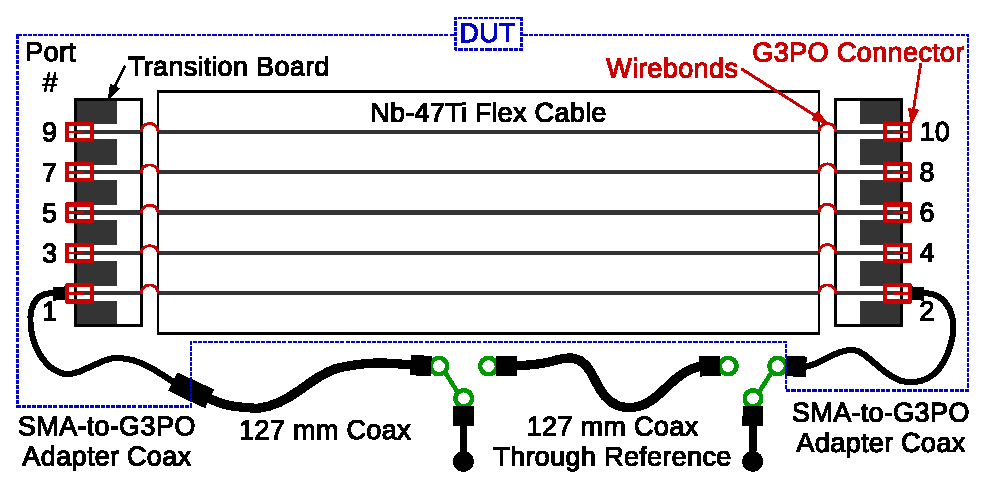
\includegraphics[width=\textwidth]{measurementDiagram2_V3.eps}
    \caption[Flex cable measurement diagram]{Diagram of the $S_{21}$ microwave measurement setup at the mixing chamber of the dilution refrigerator. The Device Under Test (DUT) consists of 203~mm Koaxis SMA-to-G3PO coaxes and the flex cable assembly including the microstrip flex circuit, wirebonds, transition boards, and G3PO edge mount connectors. Disconnected traces on the flex cable were terminated with $\rm 50~\Omega$ loads. The SMA switches allow for an in-situ through calibration without interrupting the dilution cooling cycle. $S_{41}$ is measured during a separate cool down.}
    \label{fig:Setup}
\end{figure*}

Large transmission dips appear at multiples of 420~MHz. We hypothesize power trapped in standing waves caused by the inductive impedance mismatch of the wirebonds is dissipated by dielectric losses. If this is true, the effective relative dielectric constant $\epsilon_{eff} = (c/(\lambda \cdot 420~\textrm{MHz}))^{2} = 2.6$ where the standing wave's fundamental mode wavelength, $\lambda = 2 \cdot l$, is twice the flex cable length, $l=22~\textrm{cm}$, and $c$ is the speed of light. This is consistent with empirical approximations \parencite{Wadell} from the microstrip geometry $\epsilon_{eff} \approx \frac{1}{2} \cdot (\epsilon_{r} + 1) + \frac{1}{2} \cdot (\epsilon_{r} - 1) \cdot (1 + 12 \cdot \frac{t}{w})^{-0.5} = 2.6$ where $t$ is the dielectric's thickness, $w$ is the trace width, and $\epsilon_{r}$ is the relative dielectric constant. At room temperature, Nikaflex has $\epsilon_{r}=3.5$ and the adhesive used in the dielectric stackup has $\epsilon_{r}=3.25$. 

\begin{figure*}[!t]
    \centering
      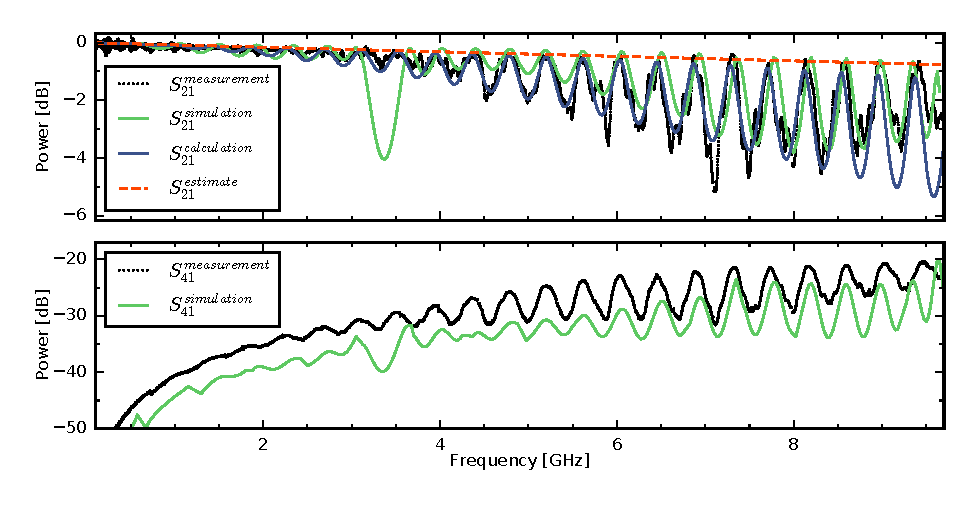
\includegraphics[width=\textwidth]{uWaveShortWB_2.eps}
    \caption[Measured transmission and crosstalk for flex cable compared to simulation]{Typical $S_{21}$ (top) and $S_{41}$ (bottom) measurements with frequency are shown of the DUT which includes the assembled flex cable and short coax cables. Blue shows the analytical model calculation of the flex cable as a transmission line with dielectric losses terminated by wirebonds as lumped element inductors. In green, we use the wirebond inductance and dielectric loss tangent estimated from the analytical calculation and simulate the response with a planar EM model in Sonnet. In red, we estimate the insertion loss without wirebonds. The calculation and simulation agree with $S_{21}$ measurements while the simulation of $S_{41}$ is systematically 2--4~dB lower than the measured values.}
    \label{fig:Measurements}
\end{figure*}

We can further substantiate this hypothesis with a 2-port analytical model where the wirebonds are represented as lumped element inductors and the superconducting flex cable is modeled by a perfectly conducting transmission line with dielectric losses (See \figurename~\ref{fig:Circuit}). By writing the ABCD matrix for each element in the model we can derive a cascade ABCD matrix for the entire network \parencite{Pozar}. The complex scattering parameter corresponding to transmission as a function of angular frequency $\omega$ is:
\setlength{\arraycolsep}{0.0em}
\begin{eqnarray}
S_{21}(\omega)&{}={}[&(Z_{f}/(2 Z_{0}) + Z_{0}/(2 Z_{f}) \nonumber\\
&&{+}\: Z_{w}^2/(2 Z_{0} Z_{f}) + Z_{w}/Z_{f}) \sinh{\gamma l} \nonumber\\
&&{+}\:(Z_{w}/Z_{0} + 1) \cosh{\gamma l}]^{-1}
\end{eqnarray}
\setlength{\arraycolsep}{5pt}
with $Z_{0}=50~\Omega$ ports, the purely imaginary wirebond impedance $Z_{w}=i \omega L$, and the complex propagation constant $\gamma = \omega \sqrt{\epsilon_{eff}} (\tan{\delta} + 2 i)/(2 c)$. From time domain reflectometry measurements we determine the flex cable's impedance $Z_{f}$ is very close to $50~\Omega$. We used a least-squares fit to match the DUT's transmission data with two free parameters, wirebond inductance $L$, and the flex cable's average dielectric loss tangent $\tan{\delta}$. The best fit plotted in \figurename~\ref{fig:Measurements} uses $L=1.0~\textrm{nH}$ and $\tan{\delta} =0.0015$. Removing the inductive impedance mismatch in the model gives an insertion loss of 0.6~dB at 8~GHz. 

We are unable to independently measure the resistive losses from the copper adapter coaxes which may be significant and calculations from first principles are insufficiently accurate due to the uncertainty in the adapter coax's copper purity. Thus, the flex cable's dielectric loss tangent may actually be much smaller than $0.0015$ since the two port analytical toy model ignores effects from the copper adapter coax, G3PO connector, copper transition board, and cross coupling to neighboring traces. This upper bound appears small considering the room temperature loss tangents of Kapton $\tan{\delta}=0.003$ and the bondplys $\tan{\delta}=0.03$. \textcite{Tuckerman} found in a similar measurement the room temperature dissipation factor for polyimides PI-2611 and HD-4100 was suppressed by a factor of a hundred at 20~mK. 

\begin{figure}[!t]
    \centering
      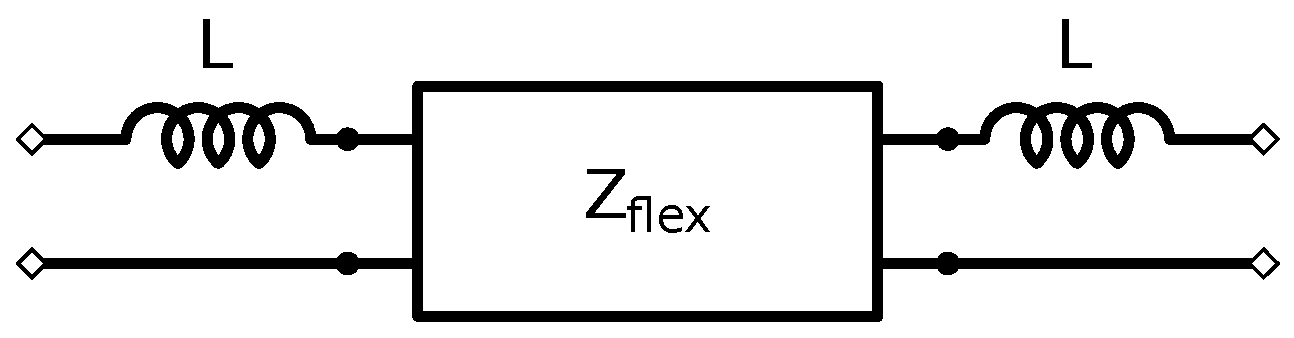
\includegraphics[width=8.5cm]{equivalentCircuit.eps}
    \caption[Equivalent circuit for flex cable]{Schematic of a single trace of the flex cable assembly as a two port equivalent circuit. The flex cable is modeled as a perfectly conducting transmission line with dielectric losses and the wirebonds are modeled as lumped element inductors with inductance L. We ignore additional components of the DUT including the copper transition board, G3PO connectors, and SMA-to-G3PO adapter coaxes.}
    \label{fig:Circuit}
\end{figure}

We use Sonnet EM software tools to model the transmission and estimate the crosstalk from the more complicated multi-port circuit. The simulation applied the $\tan{\delta} =0.0015$ and lumped element $1.0~\textrm{nH}$ inductors to match the results of the analytical calculation. While the transmission magnitude and oscillations agreed, we found the nearest neighbor crosstalk measured was 2--4~dB worse than the estimate from the Sonnet simulation. This may be because the transition board for the G3PO coaxial interface was ignored in the simulation. Sonnet is a planar simulator so accurately modeling the transition circuit becomes computationally expensive due to its inherent 3D nature. 

\subsection{Heat Flow Calculations} \label{sec:thermal}
The thermal conductance of the flex cable is calculated from literature values of the thermal conductivity of Nb-47Ti \parencite{DaalInPrep, Olson1993} and Nikaflex \parencite{Kellaris} and their respective cross sections. We assume that the Hanwha HGB adhesive has the same thermal conductivity as Nikaflex since it is similar to the epoxy that dominates the thermal conductivity in Nikaflex. In \figurename~\ref{fig:Heat} we show the calculated thermal properties per trace of our flex cable compared to the measured commercially fabricated superconducting cables from Coax Co., LTD. 

\begin{figure}[!t]
    \centering
      \includegraphics[width=9.5cm]{thermalConductance_2.eps}
    \caption[Thermal conductivity of flex cable]{We integrate the thermal conductivity over the cross sectional area as a proxy for thermal conductance, G, independent of cable length. This work calculates values per trace of the Nb-47Ti flex cables from literature values of constituent materials \parencite{DaalInPrep, Olson1993, Kellaris}. This can be compared to the directly measured conductance of the smallest commercially available superconducting Nb-47Ti coax cables from Coax Co., LTD. We show here their $\oslash$ 1.6~mm Nb-47Ti Coax (SC-160/50-NbTi-NbTi)\parencite{Kushino} and their $\oslash$ 0.86~mm diameter version (SC-086/50-NbTi-NbTi)\parencite{Kushino2016}. The dashed portion of the lines indicate data extrapolation to the temperature range of interest.}
    \label{fig:Heat}
\end{figure}

The heat load can be calculated from values in \figurename~\ref{fig:Heat} by integrating over temperature and dividing by cable length. For our 5 trace, 22~cm long, 1.8~cm wide, 0.198~mm-thick flex cable we estimate a thermal load of 60~nW on the 0.1~K ADR stage if the cable spans 11~cm from the 0.8~K stage. This is roughly equivalent to five of the 0.86~mm Nb-47Ti coaxes from Coax Co. The 0.096~mm thick flex cable is half this. Table \ref{tab:Heat} compares the thermal load from the flex cables and Coax Co.'s superconducting coax cables. 

\begin{table}[!t]
  %\renewcommand{\arraystretch}{1.3}
  \centering
  \caption[Summary of thermal, mechanical, and microwave properties for the Nb-47Ti flex cable]{Summary of Thermal, Mechanical, and Microwave Properties of the {\upshape Nb-47Ti} Flexible Microstrip Cables Presented in This Section Compared to the Best Commercially Available {\upshape Nb-47Ti} Coax Cables from {\upshape Coax Co., LTD}. The Size Indicates the Total Thickness of the Flex Cable or Outer Diameter of the Coax Cable. The Thermal Load with Cable Length per Trace is Calculated for Cables Spanning 4~K to 0.8~K and Cables From 0.8~K to 0.1~K. Measurements of the Insertion Loss and Crosstalk are Described in Section \ref{sec:measurements}. The Estimated Insertion Loss for the {\upshape 0.198~mm} Thick {\upshape Nb-47Ti} Flex Cable Gives our Model Estimate When the Wirebond Impedance Mismatch in the Assembled Flex Cable is Removed. We Have Not Measured the Microwave Properties of the Thinner {\upshape Nb-47Ti} Flex Cables. \vspace{5pt}}
  \label{tab:Heat}
  
  \begin{tabular}{ l@{\hspace{2pt}}  l@{\hspace{0cm}}  l@{\hspace{4pt}}  c  c  c@{\hspace{0cm}}  c  c  }
  \hline
  & & & \multicolumn{2}{c}{Nb-47Ti Flex} & & \multicolumn{2}{c}{Nb-47Ti Coax$^{\rm a}$} \\ \cline{4-5} \cline{7-8}
  \multicolumn{3}{l}{Size [mm]} & 0.198 & 0.096 & & $\oslash$1.6 & $\oslash$0.86 \\
  \multicolumn{3}{l}{Trace Pitch [mm]} & 3.556 & 3.556 & & $>$13 & $>$13 \\
  \multicolumn{3}{l}{Min Inside Bend Radius [mm]} & 6.4 & 3.2 & & 6.4 & 3.2 \\
  \multirow{2}{*}{\shortstack[l]{Thermal Load per\\ Trace [\SI{}{\micro\watt\centi\metre}]}} &
  	\multirow{2}{*}{\fontsize{18}{10}\selectfont \{ } & 
    0.8 K Stage & 8.4 & 2.8  & & 26. & 7.1 \\
  & & 0.1 K Stage & 0.13 & 0.07 & & 0.51 & 0.13 \\
  \multirow{2}{*}{\shortstack[l]{Insertion Loss at\\ 8~GHz [dB/m]}} &
  	\multirow{2}{*}{\fontsize{18}{10}\selectfont \{ } & 
    Measured & $<$11.4 & -- & & $<$0.4 & $<$0.5 \\
  & & Estimated & $<$2.7 & NA & & NA & NA \\
  \multicolumn{3}{l}{Crosstalk at 8 GHz [db]} & -25. & -- & & NA & NA \\
  \hline
  \end{tabular}\\
  \begin{itemize}
  \item[] $^{\rm a}$Data from Coax Co catalog: \url{http://www.coax.co.jp/en/wcaxp/wp-content/themes/coax/pdf/cryogenic_cable_catalogue.pdf}.
  \end{itemize}
\end{table}

\subsection{Conclusions on the Micrwave Wiring and Future Work}
We fabricated scalable superconducting flexible microwave push-on cables  for 10,000+ sensor MKID arrays being developed at UCSB. They could be useful in a wide variety of sub-kelvin applications with highly sensitive devices that require a large number of and tightly packed microwave feedthroughs capable of large and overlapping bandwidth. While for these prototypes we use a panel manufacturing process, the fabrication technique of laminating Nb-47Ti foil to a polyimide substrate and wet etching is amenable to a roll-to-roll manufacturing process for very long flexible cables. The thermal conductance below 4~K for the 0.198~mm thick Nb-47Ti flex cable is roughly equivalent per trace to the smallest ($\oslash$0.86 mm) Nb-47Ti coax cables from Coax Co.. The second iteration of the flex cable is only 0.096~mm thick and will have half the thermal load. In either event, an ADR's thermal budget can be accommodated by increasing the flex cable's length.

We found an average insertion loss of $<$2.7 dB/m at 8~GHz for the 22~cm long, 0.198~mm-thick flex cable assuming the impedance mismatch caused by the wirebonds can be removed. This loss is more than five times the measured insertion loss for commercially available superconducting Nb-47Ti coax cables from Coax Co. which cannot be explained by the different cable geometry. The loss is likely do to an unknown combination of factors including the uncorrected loss from the copper adapter coaxes in the DUT, and a difference in the dielectric loss properties of Kapton and Teflon below 1K which are unexplored in literature.

Several avenues exist to avoid the impedance mismatch including a better transition board design or plating of the Nb-47Ti with a solderable metal like copper or aluminum. The plating technique is especially desirable because it would remove the need for a transition board and enable the fabrication of via structures and therefore more complicated multilayer designs such as stripline. The greater isolation enjoyed by the stripline structure over microstrip could be used to improve the cross talk between traces, although the measured -25~dB nearest neighbor cross talk is sufficiently low for our current MKID applications. Additionally, the 0.096~mm thick flex cable fabricated will have improved cross talk performance due to the thinner traces and their closer proximity to the ground plane. 